% !TeX encoding = UTF-8
%% (requires IEEEtran.cls version 1.7 or later) with an IEEE conference paper.
\documentclass[conference]{IEEEtran}


% *** GRAPHICS RELATED PACKAGES ***
%\usepackage[pdftex]{graphicx}
\usepackage{graphicx}
%\usepackage[dvips]{graphicx}
% to place figures on a fixed position
\usepackage{float}

% *** PDF, URL AND HYPERLINK PACKAGES ***
\usepackage{url}

% correct bad hyphenation here
%\hyphenation{}

\usepackage{xcolor}


\newcommand\note[1]{\textcolor{red}{#1}}
% \renewcommand\note[1]{} % uncomment this line to hide notes

%%%%%%%%%%%%%%%%%%%%%%%%%%%%%%%%%%%%%%%%%%%%%%%%%%%
%%%%%%%%%%%%%%%%%%%%%%%%%%%%%%%%%%%%%%%%%%%%%%%%%%%
%%%%%%%%%%%%%%%%%%%%%%%%%%%%%%%%%%%%%%%%%%%%%%%%%%%
%


% LaTeX quick ref
%
% \cite{refname} to place citation
%
% \label{label_name} to place a label, which can be reference by \ref{label_name}
%
% new paragraph -> empty line between text
%
% \noindent to not indent paragraphs first line
%
% create list with : \begin{itemize} \end{itemize}
% \begin{itemize
% \renewcommand to renew numbering \labelitemi{--} to select bullet type
% \item item elem 1
% \item item elem2
% \end{itemize}
%
% et alia (et al.) should be emphasized (i.e in italic) with \emph{et al.}
%
% to add figure, htb is placement selector , !overrid internal paramters
%\begin{figure}[!htb]
%    \centering
%    \includegraphics[width=9cm]{FIG.png}
%    \caption{Caption}
%    \label{fig:label}
%\end{figure}
%
% ~ concatenates dynamic text with literals
%
% long dash is --
%
% `is single quoted' , ``is double qouted"



\begin{document}


% conference papers do not typically use \thanks and this command
% is locked out in conference mode. If really needed, such as for
% the acknowledgment of grants, issue a \IEEEoverridecommandlockouts
% after \documentclass
% paper title
% can use linebreaks \\ within to get better formatting as desired
\title{Protocol Implementations using FPGAs}
% author names and affiliations
% use a multiple column layout for up to three different
% affiliations
\author{\IEEEauthorblockN{Ferenc Nandor Janky}
\IEEEauthorblockA{Dept. of Telecommunications and MediaInformatics\\Technical University of Budapest\\Budapest, Hungary\\
Email: fecjanky@gmail.com}
}


% make the title area
\maketitle


\begin{abstract}
\boldmath
The handling of connectionless networking protocol messages with low memory utilization could be achieved effectively by using FPGAs. When lower level protocols are implemented in such way, they will provide fast and predictable service characteristics for their upper layer protocols. The perturbation of their software implemented variants such as delay and jitter could be eliminated using the pure hardware implementaion of the operation. One of the key factors of the mentioned side effects is the hosting operating system’s scheduling algorithm.
The purpose of this \dots was to design a generalized approach for implementing protocols using FPGA hardware, and to validate the theory by implementing an application layer protocol using the resulting framework.
The OSI Basic Reference Model is a remarkable guideline as a design basis for setting the boundaries of such framework, because it’s purpose is to provides a common basis for the coordination of standards development for the purpose of systems interconnetion.
As a result of this work the designed framework has been described in VHDL. It follows the basic principles of the OSI reference presenting a general toolkit for handling  PDUs and IDUs beside these features it also provides solutions for other frequently reappearing tasks in the aid of convenient and smoother implementation of various systems interconnecting protocols.
To verify the design a partial implementation of SNMP and various other lower layer protocols have been implemented which was interconnected with with other link, network and transport layer hardware and software products from 3rd party vendors. The conformance testing of the SNMP implementation had been carried out with a couple of network management software.

\end{abstract}


% no keywords



\section{Motivation}\label{sec:Motivation}

The family of connectionless low memory footprint networking protocols can be handled with relative ease by having pure hardware based implementations using FPGAs. One of the biggest motivation of having hardware based protocol implementations is to provide deterministic timing characterisitcs which is essential for several newtorking protocols such as Time Triggered Ethernet~\cite{SAE_AS6802} whereas time synchronization protocols like PTP could also benefit from them. Most FPGA manufacturers provide black box modules of which several protocols can be synthetized however the problematic part is that for academic purposes where most often non-existing features or protocols have to be implemented those are not suitable because often only some generic parameters of a given protocol can be tweaked as a part of instantiation. The motivation for this work is to design and implement a framework in VHDL which enables rapid prototyping of networking protocols. The aim is not to provide similar black box modules but to supply elementary components in a way that the implementor could only focus in desinging and implementing the protocol specific parts. The ISO OSI model provides a standard way of talking about protocols as a result lining up the design of the framework with the OSI model is a straightforward decision. Beside that it provides well established nomenclature it also lays down the fundamentals of the modular architecture of the framework.

\section{Related Work}\label{sec:RelatedWork}

TODO: read papers and provide summary

introduce some related works (at least three), from papers 

\section{Internal Design}\label{sec:Internal Design}

As introduced in \ref{sec:Motivation} the internal design of the framework aligns with the OSI model. Individual layers of protocols communicate through SAPs using service primitives which mostly have protocol dependent parameters but its sturcture is fixed and consists of ICI and SDU. Given these it's benefitial to have a component which can be reused in each and every protcol for handling ICIs SDUs and PDUs. The implementor's task is to:
\begin{itemize}
\renewcommand \labelitemi{--}
\item implement the protocol operation as specified
\item implement interface towards upper layer protocols
\item implement interface towards lower layer protocols
\end{itemize}

Based on the description above the framework in itself is module/building block which has the follwing properties: 

\begin{itemize}
\renewcommand \labelitemi{--}
\item the fundamental building block of the framework has to support interconnection via layering
\item handle reception and transmission of PDUs with queuing 
\item provide a high level interface for separating and combining PCI and SDU, forwarding pausing or dropping SDUs
\item provide a unified way to handle ICI SDU and PDU events (e.g error signalling)
\item add support of auxilliary information that travels along with messages -- this can be used for adding metadata to message or in implementing ceratin SAPs
\item provide components for common tasks reocurring during impelementing networking protocols (de/serialization, arbitration etc.)
\end{itemize}

Figure~\ref{fig:system_sketch} shows the high level design of the Protocol Layer module. The PUI and PIP part is interconnected via a control and a data bus. The control signals provide a way for signalling various conditions: start of PDU, end of PDU, etc. All of the module's buses are configurable via generics in terms of:
\begin{itemize}
\renewcommand \labelitemi{--}
\item bus width
\item handshaked or usnolicited mode of tx/rx
\item no. of messages to queue
\item instantiate aux. queue for tx/rx
\end{itemize}

\begin{figure}[!htb]
    \centering
    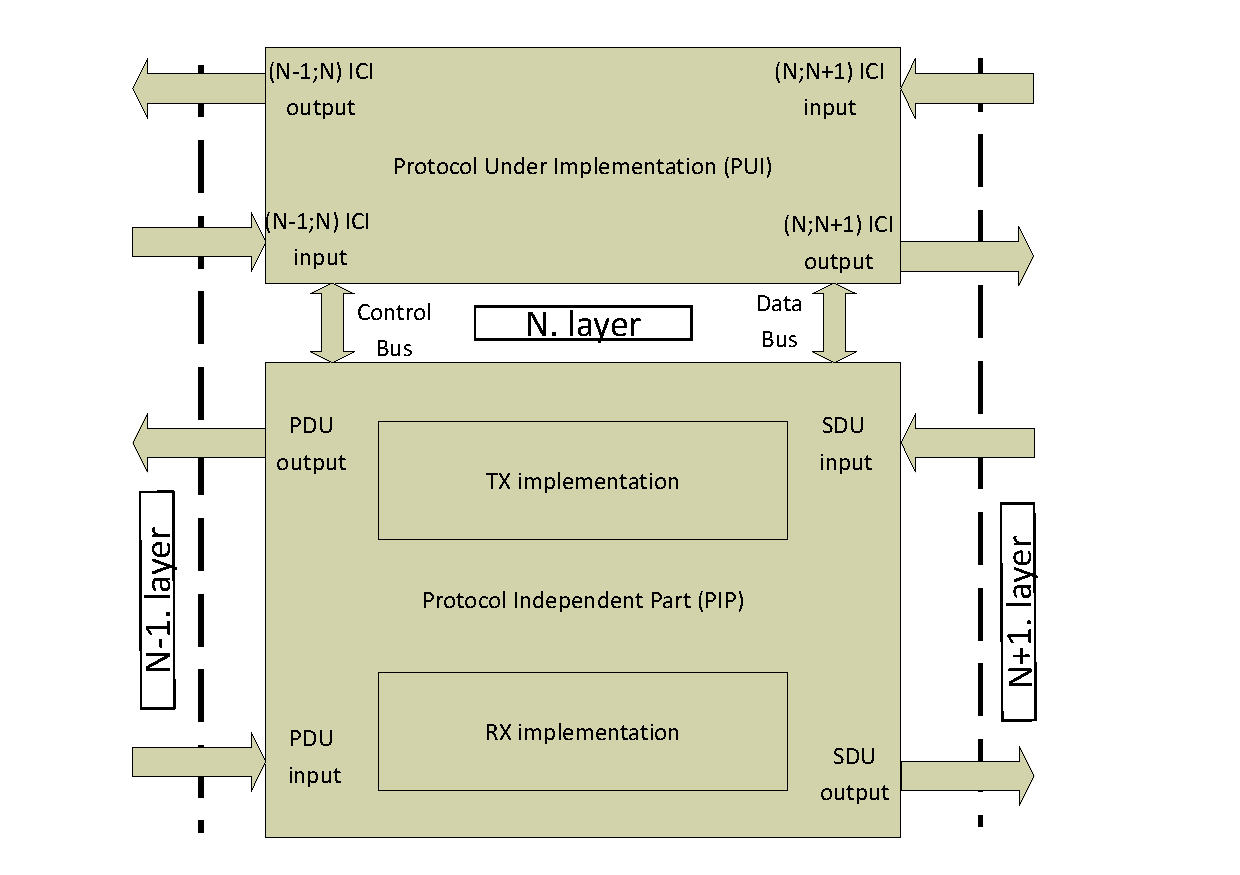
\includegraphics[width=9cm]{figures_raw/system_sketch.pdf}
    \caption{System sketch of the fundamental building block of the framework}
    \label{fig:system_sketch}
\end{figure}

\subsection{Interface and functional specification of the VHDL modules}\label{subsec:if_and_func_spec_VHDL}

\subsubsection{Handshaking mechanism and error signalling}
In synchronous systems there is a need for handshaking to indicate a request for certain operations to be carried out. In this framework this is generalized into having two signals -- \emph{Ind} for indicating a request; -- \emph{Ack} for providing acknowledegment for the requested operation. All synchronous operations must be carried out after receiving an \emph{Ack}. Synchronous operation is not always prefereable -- e.g. when there is only one upper layer protocol in a given system that is the reason why every interface is parametrizable with generics whether to use synchronization or not.
For signalling error conditions bidirectional error indicator signals are present beside the bidirectional data and control buses so that both interconnected modules can signal error conditions.

\subsubsection{Data delimiter signals}

Data is traversing through the system in the form of consequtive bytes over various data buses (PDU,internal data, aux. data etc.) accompanied by 3 control signals:
\begin{itemize}
\renewcommand \labelitemi{--}
\item Start Of PDU abbreviated as SOP
\item End of PDU abbreviated as EOP
\item Data Valid abbreviated as DV
\end{itemize}
If a module is transferring data it must indiciate it by transitioning both SOP and DV signals from logical `Low' to `High' level simultaneously and in parallel the data bus is also adjusted to the first symbol of the data to be sent. If a module samples SOP and DV on a rising edge of the clock then it can shift in and start process the data from the data bus when DV is `High' -- among other things that can be used as a write enable signal. The end of data is signalled by pulse on the EOP line while DV is `High'. After this all control signals have to be settled on `Low' logical level.

\subsubsection{Combining handshaking, error handling and delimiters}

Figure~\ref{fig:data_signals} illustrates data transfer combined with synchronization. The delimited data transfer must take place after \emph{Ind}-\emph{Ack} handshake i.e when the sending component samples `High' on the \emph{Ack} wire.  The receiver can withold the acknowledment idefinitely -- the sender must only reset the indication signal if an error is signalled. The source module can cancel the transmission by transitioning the \emph{Ind} signal back to `Low' level. After the handshake the data transmission must take place -- after a successful handshake the sender can only cancel the transmission via signalling error.

% WaveDrom waveform
%{signal: [
%  {name: 'CLK', wave: 		'P........|.....'},
%  {name: 'Ind', wave: 		'0.1..0...|.....'},
%  {name: 'Ack', wave: 		'0..1.0...|.....'},
%  {name: 'SOP', wave: 		'0...10...|.....'},
%  {name: 'EOP', wave: 		'0........|..10.'},
%  {name: 'DV', wave:  		'0...1....|...0.'},
%  {name: 'DATA[x:0]', wave: 'x...3....|...x.', data: ['data']},
%]}
\begin{figure}[!htb]
    \centering
    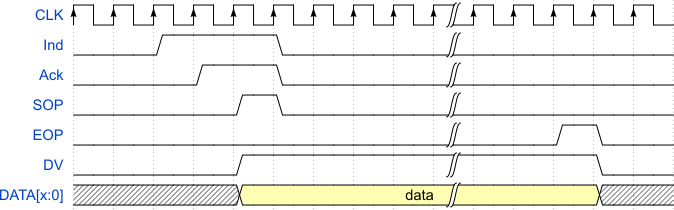
\includegraphics[width=9cm]{figures_raw/data_signals.png}
    \caption{Waveform of a typical error free data transmission between modules}
    \label{fig:data_signals}
\end{figure}



Design should follow the OSI modell, high level description and specification (p.37) of the modules + description of figures
(fig. 16,19, 20)


Explain a bit

\begin{figure}[!htb]
    \centering
    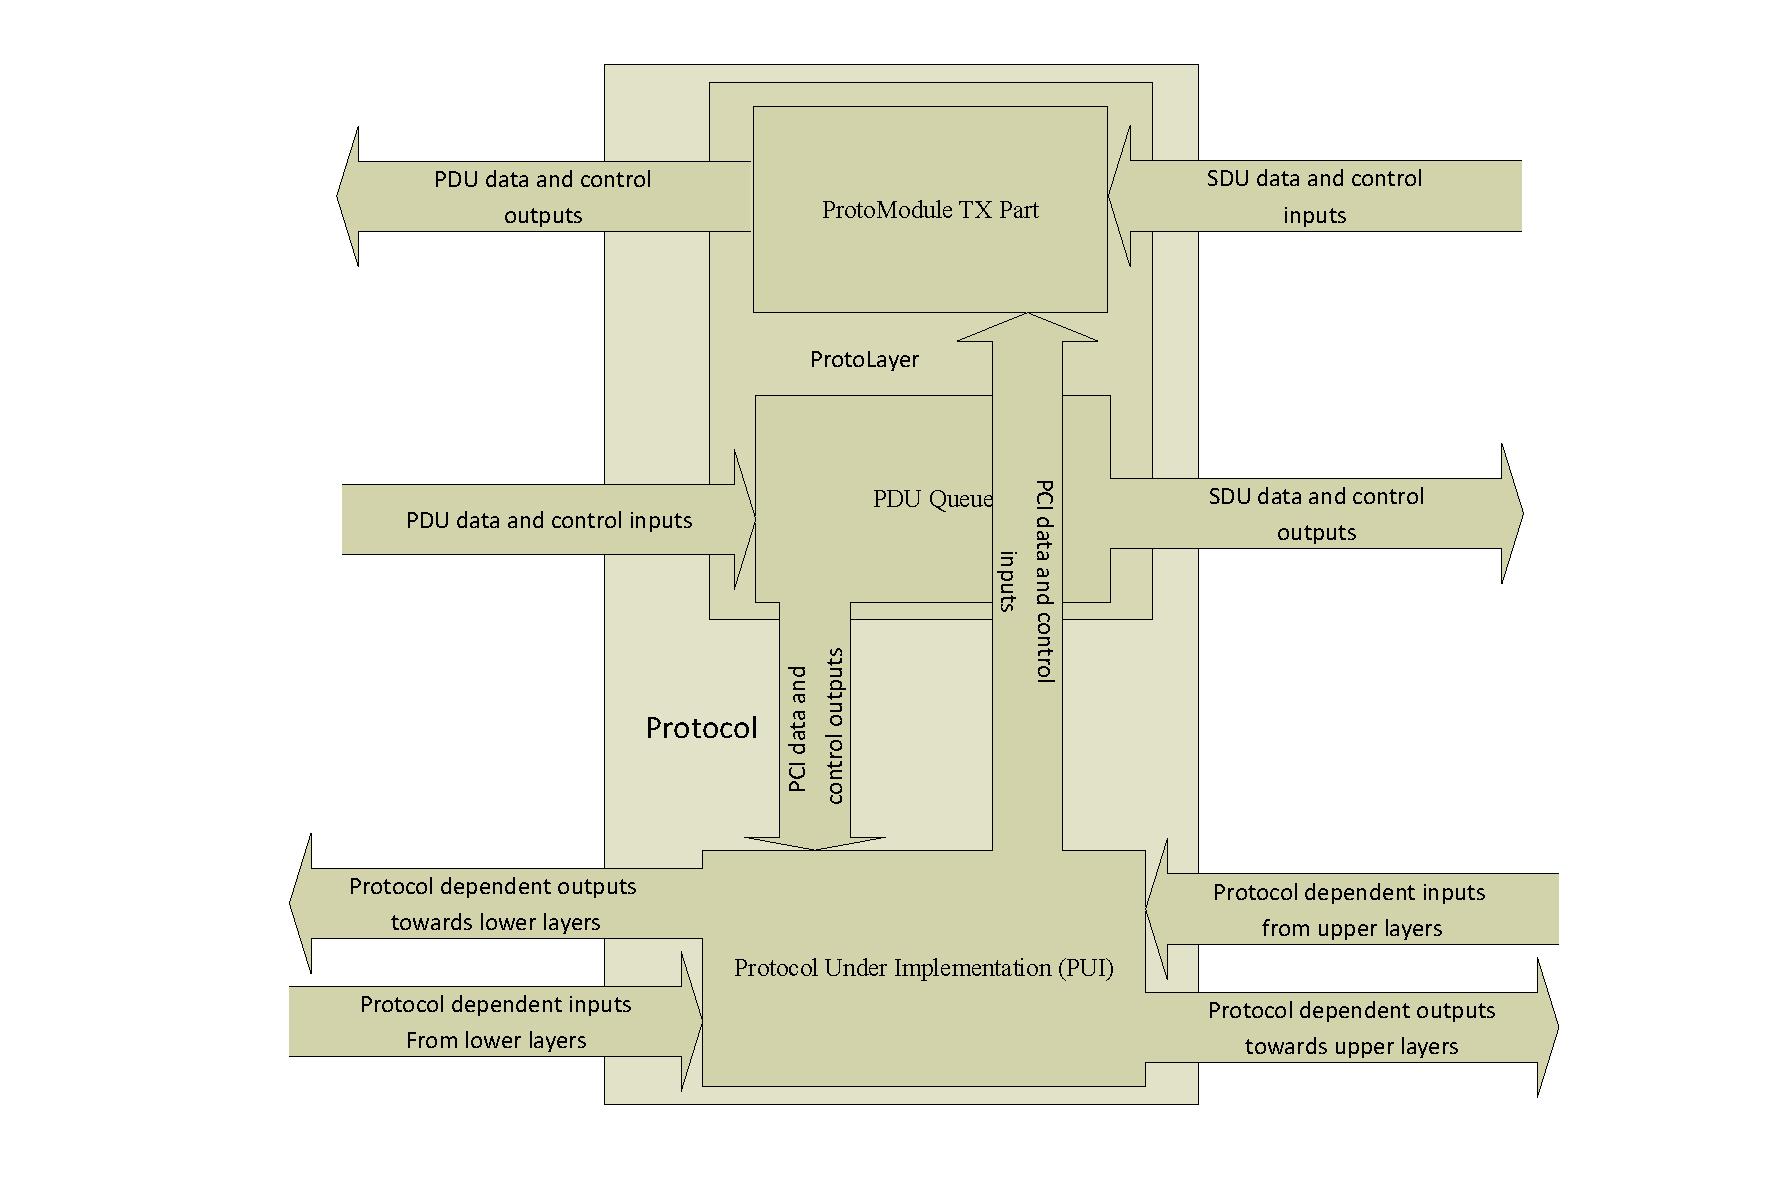
\includegraphics[width=9cm]{figures_raw/protlayer_2.pdf}
    \caption{Schematic drawing of a Protocol layer modul}
    \label{fig:proto_layer_sch}
\end{figure}

\section{Implementation}\label{sec:Implementation}

Overview of the VHDL implementation with focus on reusability and scientific value

\section{Verification}

Show results with through simualation waveforms and pcap of the generated SNMP packets

\section{Conclusion}

And summarize with a nice conclusion\cite{Williams_Web_Workload_Characterization_10_Years}

\section{Acknowledgement}
We would like to thank to all of our colleagues and students who contributed to the success of our project


% can use a bibliography generated by BibTeX as a .bbl file
% BibTeX documentation can be easily obtained at:
% http://www.ctan.org/tex-archive/biblio/bibtex/contrib/doc/
% The IEEEtran BibTeX style support page is at:
% http://www.michaelshell.org/tex/ieeetran/bibtex/

\bibliographystyle{IEEEtran}
% argument is your BibTeX string definitions and bibliography database(s)
\bibliography{references}

%
% <OR> manually copy in the resultant .bbl file
% set second argument of \begin to the number of references
% (used to reserve space for the reference number labels box)

%\begin{thebibliography}{1}
%
%\bibitem{IEEEhowto:kopka}
%H.~Kopka and P.~W. Daly, \emph{A Guide to \LaTeX}, 3rd~ed.\hskip 1em plus
% 0.5em minus 0.4em\relax Harlow, England: Addison-Wesley, 1999.
%
% \end{thebibliography}


\end{document}


